\documentclass[11pt]{article}
\usepackage[margin=1in]{geometry}
\usepackage{amsmath,amssymb,booktabs,microtype,graphicx}
\usepackage[section]{placeins}
\usepackage[round]{natbib}
\usepackage[hidelinks]{hyperref}
\graphicspath{{figures/}{figures/info_scale/}{notes/figures/info_scale/}}
\setlength{\parindent}{0pt}
\setlength{\parskip}{0.4em}
\setlength{\emergencystretch}{2em}
\raggedbottom
\newcommand{\Rhat}{\hat R}
\title{An information scale for the mixing of the Default BART sampler}
\author{}
\date{5 November 2026}

\begin{document}
\maketitle
\vspace{-1.5em}

\section{Question}
In the paper's two-budget comparison (Section~3), Default chains still disagree after $10^7$ iterations on some settings and agree on others. Sample size alone does not order the settings: Airfoil ($N=1503$) remains elevated, whereas Abalone ($N=4177$) resolves. \citet{tan2024computational} attribute slow convergence of BART samplers to large $n$ and high signal-to-noise ratio. This note asks whether the two factors act through a single quantity, and whether that quantity orders the settings used in the paper. Section~\ref{sec:long-pt} reports the long MTMH+PT chains on SeoulBike.

\section{A likelihood scale for structural moves}
\label{sec:scale}
Consider an update of tree $j$ with partial residual $r\in\mathbb R^n$, leaves $\ell$ with $n_\ell$ rows and residual sums $S_\ell$, leaf prior $N(0,\tau^2)$ and noise variance $\sigma^2$. Integrating the leaves gives
\begin{equation}
\log p(r\mid\mathcal T_j,\sigma^2) = -\frac{n}{2}\log(2\pi\sigma^2) - \frac{1}{2\sigma^2}\Bigl[\sum_i r_i^2 - \sum_\ell \frac{S_\ell^2}{n_\ell+\sigma^2/\tau^2}\Bigr] - \frac12\sum_\ell \log\Bigl(1+\frac{n_\ell\tau^2}{\sigma^2}\Bigr).
\label{eq:collapsed}
\end{equation}
When $n_\ell\gg\sigma^2/\tau^2$, the bracket is the residual sum of squares $\mathrm{RSS}(\mathcal T_j)$ after fitting leaf means. A structural proposal then changes the log likelihood by
\begin{equation}
\Delta\log p \approx -\frac{\Delta\mathrm{RSS}}{2\sigma^2} + O\Bigl(\log\frac{n_\ell\tau^2}{\sigma^2}\Bigr)\ \text{per leaf added or removed}.
\end{equation}
Write $\Delta\mathrm{RSS}=n s_y^2\,\delta$, where $s_y^2$ is the training variance of $y$ and $\delta$ is the change in the in-sample unexplained fraction. Near stationarity $\sigma^2\approx(1-R^2)s_y^2$, so
\begin{equation}
\Delta\log p \approx -\frac{\kappa}{2}\,\delta,\qquad \kappa=\frac{n}{1-R^2}=n\,(1+\mathrm{SNR}),
\label{eq:kappa}
\end{equation}
with $\mathrm{SNR}=R^2/(1-R^2)$. The tree prior ratio and the proposal ratio do not depend on $n$ or $\sigma^2$, and the leaf term grows only logarithmically. A move that worsens the fit by $\delta>0$ is therefore accepted with probability at most of order $\exp(-\kappa\delta/2)$, up to factors that do not depend on $\kappa$.

A change in the decomposition of the ensemble generally passes through intermediate states with a worse fit. If the required loss $\delta^\ast$ is similar across datasets, the crossing rate decreases like $\exp(-\kappa\delta^\ast/2)$, and $\kappa$ sets the difficulty. For $\delta^\ast=10^{-4}$, the cost is $0.28$ nats on Abalone ($\kappa\approx5.6\times10^3$), $3.1$ nats on SeoulBike ($\kappa\approx6.3\times10^4$) and $18$ nats on CPU activity ($\kappa\approx3.6\times10^5$). Tempering at temperature $T$ replaces $\kappa$ by $\kappa/T$.

The argument makes two testable predictions:
\begin{enumerate}
\item $\kappa$ orders mixing difficulty across datasets better than $n$ or $1-R^2$ separately.
\item In a regression of a mixing diagnostic on $\log n$ and $\log\{1/(1-R^2)\}$, the two coefficients are equal.
\end{enumerate}

\section{Settings and measurements}
\textbf{Settings (48).}
\begin{itemize}
\item The twelve paper settings, with five runs each. The three DART settings use the Default sampler with the Dirichlet splitting prior, as in the paper.
\item The 20 size and noise sweep settings of Section~3, with five runs each.
\item 16 controlled settings on SeoulBike, Airfoil and Abalone, with three runs each, using the store train splits 0--2 and fixed test panels. These keep $X$ and $n$ fixed and replace the response by one of three choices:
\begin{itemize}
\item the observed $y$;
\item $y$ plus independent Gaussian noise;
\item a semi-synthetic response $\hat f(X)+\varepsilon$, with $\varepsilon$ Gaussian and homoskedastic. Here $\hat f$ is a histogram gradient boosting fit (500 iterations) to the full dataset, used as a known regression function.
\end{itemize}
Noise variances are set to reach the target noise fractions in Table~\ref{tab:controlled}.
\end{itemize}

\textbf{Mixing diagnostic.} The rank-normalized split $\Rhat$ (ArviZ, as in the paper) is computed at each of the 100 fixed test inputs from four Default chains. As in the paper, every record keeps 7,000 post-warm-up draws per chain:
\begin{itemize}
\item $10^4$-iteration chains: iterations 3,001--10,000;
\item $10^7$-iteration chains: the last 70\% of the stride-1,000 record.
\end{itemize}
The note reports the median over inputs, averaged over runs.

\textbf{Noise fraction.} $1-R^2_{\mathrm{CV}}$ is the 5-fold cross-validated mean squared error of histogram gradient boosting on the training set, divided by $s_y^2$. It requires no MCMC. The posterior alternative is $\bar\sigma^2/s_y^2$, computed from the same retained Default draws; correlations with both are reported.

\textbf{Acceptance rates.} One Default chain per setting (run 0) is used. The acceptance rate is the number of accepted proposals divided by the number of valid proposals, over iterations $3{,}001$--$5{,}000$.

\section{Results}
\subsection{Ordering across settings}
Figure~\ref{fig:kappa}(a) plots $\Rhat-1$ against $\kappa$ for all 48 settings, and Table~\ref{tab:spearman} gives the rank correlations. $\kappa$ gives $\rho=0.89$, compared with $0.66$ for $n$ and $0.60$ for $1/(1-R^2_{\mathrm{CV}})$. On the twelve paper settings at $10^7$ iterations, $\rho=0.86$ for $\kappa$ and $0.57$ for $n$.

Table~\ref{tab:paper} lists the paper settings by $\kappa$:
\begin{itemize}
\item Airfoil and Abalone, which have similar $N$ but opposite outcomes, differ threefold in $\kappa$.
\item CalHousing, Friedman and Airfoil have nearly equal $\kappa$ and similar $10^4$-iteration $\Rhat$.
\item The four settings that remain above $1.1$ after $10^7$ iterations have the four largest values of $\kappa$.
\item The three DART settings share $n$ and the noise level with Friedman. Their posterior noise fraction is the same ($0.037$ against $0.036$), and their $\Rhat$ is close to Friedman's (1.17--1.20 against 1.23). Their cross-validated $\kappa$ is lower (1.2--1.6$\times10^4$) because the gradient-boosting error grows with the number of nuisance predictors.
\end{itemize}

\begin{table}[h]
\centering
\caption{Spearman correlation of median pointwise $\Rhat$ with candidate scales.}
\label{tab:spearman}
\begin{tabular}{lccc}
\toprule
Scale & 48 settings, $10^4$ its & 48 settings, $10^4$ its & 12 paper settings, $10^7$ its \\
 & ($1-R^2_{\mathrm{CV}}$) & ($\bar\sigma^2/s_y^2$) & ($1-R^2_{\mathrm{CV}}$) \\
\midrule
$\kappa=n/(1-R^2)$ & 0.89 & 0.89 & 0.86 \\
$n$ & 0.66 & 0.66 & 0.57 \\
$1/(1-R^2)$ & 0.60 & 0.44 & 0.42 \\
\bottomrule
\end{tabular}
\end{table}

\begin{table}[h]
\centering
\caption{Paper settings ordered by $\kappa$. $n$ is the training size; $\Rhat$ is the median pointwise value averaged over five runs. The last column gives the acceptance rate of change moves.}
\label{tab:paper}
\begin{tabular}{lrrrccc}
\toprule
Setting & $n$ & $1-R^2_{\mathrm{CV}}$ & $\kappa$ & $\Rhat$, $10^4$ & $\Rhat$, $10^7$ & change acc. \\
\midrule
Abalone & 3{,}057 & 0.543 & 5{,}629 & 1.097 & 1.000 & 0.163 \\
Concrete & 697 & 0.083 & 8{,}436 & 1.173 & 1.003 & 0.136 \\
DART $d{=}200$ & 1{,}425 & 0.117 & 12{,}219 & 1.184 & 1.000 & 0.099 \\
DART $d{=}100$ & 1{,}425 & 0.107 & 13{,}327 & 1.173 & 1.000 & 0.088 \\
DART $d{=}20$ & 1{,}425 & 0.091 & 15{,}644 & 1.199 & 1.000 & 0.104 \\
Friedman & 1{,}425 & 0.083 & 17{,}217 & 1.233 & 1.002 & 0.136 \\
Airfoil & 1{,}052 & 0.060 & 17{,}420 & 1.298 & 1.041 & 0.112 \\
CalHousing & 3{,}675 & 0.205 & 17{,}958 & 1.251 & 1.018 & 0.105 \\
Superconduct & 3{,}675 & 0.139 & 26{,}517 & 1.441 & 1.234 & 0.062 \\
SeoulBike & 6{,}495 & 0.103 & 62{,}812 & 1.466 & 1.318 & 0.061 \\
CCPP & 7{,}101 & 0.036 & 194{,}668 & 1.439 & 1.126 & 0.043 \\
CPU activity & 6{,}069 & 0.017 & 364{,}149 & 1.518 & 1.236 & 0.031 \\
\bottomrule
\end{tabular}
\end{table}

\begin{figure}[h]
\centering
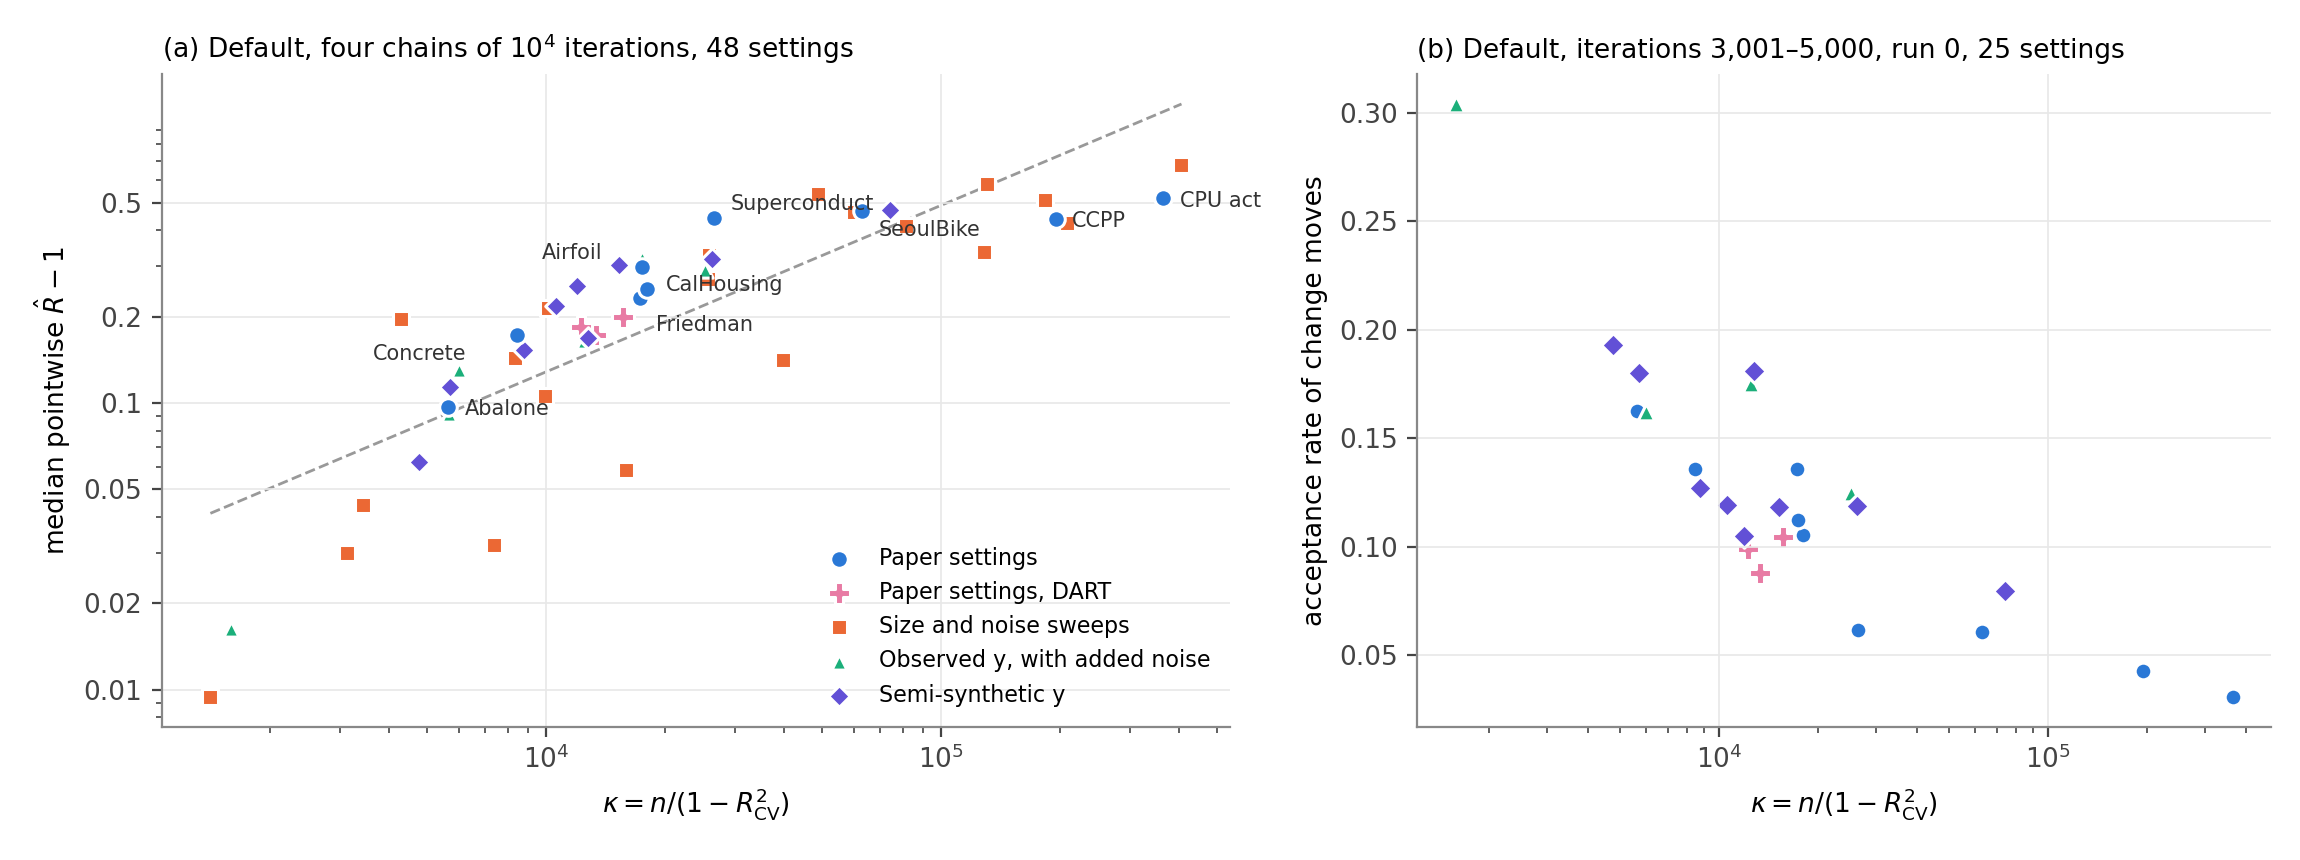
\includegraphics[width=\linewidth]{rhat_vs_kappa.png}
\caption{(a) Median pointwise $\Rhat-1$ against $\kappa$ for 48 settings, on logarithmic axes. The dashed line is the least-squares fit $\log(\Rhat-1)=0.58\log\kappa-7.40$. (b) Acceptance rate of Default change moves against $\kappa$, one chain per setting; markers as in (a).}
\label{fig:kappa}
\end{figure}

\subsection{Do $n$ and the noise fraction enter only through $\kappa$?}
Over the 48 settings, fit the regression
\[
\log(\Rhat-1)=a\log n+b\log\{1/(1-R^2)\}+c .
\]
With $1-R^2_{\mathrm{CV}}$ it gives $a=0.61\pm0.08$ and $b=0.55\pm0.09$. With $\bar\sigma^2/s_y^2$ it gives $a=0.72\pm0.08$ and $b=0.55\pm0.07$, a gap of about 1.6 combined standard errors. The standard errors are from ordinary least squares.

Constraining $a=b$, that is regressing on $\log\kappa$ alone, barely changes the coefficient of determination: 0.68 versus 0.68 with $1-R^2_{\mathrm{CV}}$, and 0.71 versus 0.73 with $\bar\sigma^2/s_y^2$. By comparison, $\log n$ alone gives 0.40 and $\log\{1/(1-R^2_{\mathrm{CV}})\}$ alone gives 0.32. Within this range, a change in $n$ and a change in the noise fraction have nearly the same effect when they change $\kappa$ by the same factor.

\subsection{Observed and semi-synthetic responses}
Table~\ref{tab:controlled} holds $X$ and $n$ fixed. At matched noise fractions, the observed response and the semi-synthetic response give nearly equal $\Rhat$:
\begin{itemize}
\item SeoulBike: 1.484 and 1.472; 1.291 and 1.318; 1.165 and 1.168;
\item Airfoil: 1.321 and 1.303; 1.130 and 1.114.
\end{itemize}
The semi-synthetic response is homoskedastic, Gaussian and has a known regression function. Features of the observed responses, such as count-valued and heteroskedastic SeoulBike rentals, are therefore not needed to produce the observed disagreement. The value of $\kappa$ suffices.

For Abalone, $\hat f$ contains structure that 3,057 rows do not identify. The attainable $1-R^2_{\mathrm{CV}}$ therefore stays near 0.26 at the smallest design noise. Measured by the attainable $\kappa$, these settings follow the same ordering.

\begin{table}[h]
\centering
\caption{Controlled settings: mean over three runs; acceptance from run 0. ``Target'' is the design noise fraction.}
\label{tab:controlled}
\begin{tabular}{llcccrc}
\toprule
Data & Response & Target & $1-R^2_{\mathrm{CV}}$ & $\kappa$ & $\Rhat$, $10^4$ & change acc. \\
\midrule
SeoulBike & observed & -- & 0.102 & 63{,}553 & 1.484 & 0.061 \\
SeoulBike & semi-synthetic & 0.042 & 0.088 & 73{,}993 & 1.472 & 0.079 \\
SeoulBike & observed + noise & 0.17 & 0.258 & 25{,}218 & 1.291 & 0.125 \\
SeoulBike & semi-synthetic & 0.17 & 0.247 & 26{,}320 & 1.318 & 0.119 \\
SeoulBike & observed + noise & 0.4 & 0.520 & 12{,}484 & 1.165 & 0.175 \\
SeoulBike & semi-synthetic & 0.4 & 0.509 & 12{,}755 & 1.168 & 0.181 \\
\midrule
Airfoil & observed & -- & 0.060 & 17{,}434 & 1.321 & 0.112 \\
Airfoil & semi-synthetic & 0.025 & 0.069 & 15{,}242 & 1.303 & 0.118 \\
Airfoil & observed + noise & 0.1 & 0.175 & 6{,}004 & 1.130 & 0.162 \\
Airfoil & semi-synthetic & 0.1 & 0.184 & 5{,}709 & 1.114 & 0.180 \\
Airfoil & observed + noise & 0.4 & 0.663 & 1{,}586 & 1.016 & 0.304 \\
\midrule
Abalone & observed & -- & 0.540 & 5{,}666 & 1.092 & 0.163 \\
Abalone & semi-synthetic & 0.38 & 0.642 & 4{,}760 & 1.062 & 0.193 \\
Abalone & semi-synthetic & 0.1 & 0.348 & 8{,}784 & 1.153 & 0.127 \\
Abalone & semi-synthetic & 0.04 & 0.288 & 10{,}600 & 1.217 & 0.119 \\
Abalone & semi-synthetic & 0.01 & 0.256 & 11{,}958 & 1.255 & 0.105 \\
\bottomrule
\end{tabular}
\end{table}

\subsection{Acceptance rates}
Equation~\eqref{eq:kappa} implies that, at stationarity, a larger share of proposals is rejected as $\kappa$ grows. Over the 25 paper and controlled settings with measured rates, Spearman correlations with $\kappa$ are $-0.80$ (grow), $-0.75$ (prune), $-0.79$ (change) and $-0.73$ (swap). Change-move acceptance falls from 0.30 at $\kappa\approx1.6\times10^3$ to 0.03 at $\kappa\approx3.6\times10^5$ (Figure~\ref{fig:kappa}(b)). At fixed $X$, adding noise raises every rate; on SeoulBike, change acceptance rises from 0.061 to 0.175.

\section{Long MTMH+PT chains on SeoulBike}
\label{sec:long-pt}
\textbf{Setup.}
\begin{itemize}
\item Data: SeoulBike, run 0, with the same training split and fixed test panel as the short chains.
\item Chains: four independent MTMH+PT chains ($K=10$) of $10^6$ iterations each.
\item Tempering: the 46-temperature run-0 ladder of the short-chain search ($T$ from 1 to 100), exchanges every 50 iterations, one worker per temperature.
\item Execution: each chain runs in 100 chunks of $10^4$ iterations, and each chunk continues from the final states of the previous one. Seeds follow the long-chain convention $2024+100{,}000+\text{chain}$; the code is commit \texttt{e86f19d}.
\item Records: two, as for the $10^7$-iteration Default chains.
\begin{itemize}
\item Thinned record: every 100th cold-replica draw, $10^4$ per chain. After the first 30\% is discarded, it holds 7,000 draws spread over 700,000 iterations.
\item Consecutive tail: the final $10^4$ iterations at stride 1, of which the last 7,000 are retained.
\end{itemize}
Each thinned draw also records $\sigma$, split counts and the collapsed log posterior at $T=1$.
\item Cost: a chunk took 763--909\,s on 47 cores, about 23\,h per chain.
\end{itemize}

\textbf{Budget.} The paper measures cost in units of the production wall time of one Default chain of $10^4$ iterations, with one worker per temperature for PT (Section~6.3 of the paper). On SeoulBike one MTMH+PT chain of $10^4$ iterations costs 8.39 units. A chain of $10^6$ iterations therefore costs about $100\times8.39\approx840$ units, against $1{,}000$ units for a Default chain of $10^7$ iterations. The two long records thus have comparable wall time, with the MTMH+PT chains about 16\% cheaper. The comparison is in wall time only: the tempered chains run 46 replicas in parallel and use up to about 39 times as many core-hours.

\textbf{Agreement.} Table~\ref{tab:long-pt} compares run-0 diagnostics, each from 7,000 draws per chain.
\begin{itemize}
\item On the thinned record, the long MTMH+PT chains give a median pointwise $\Rhat$ of 1.239. This is lower than Default at either budget (1.504 and 1.310) and close to the production MTMH+PT and Default+PT chains (1.225 and 1.170).
\item It remains far from agreement: 99\% of inputs exceed 1.01 and 77\% exceed 1.1. For the log posterior $\Rhat$ is 1.51, and for $\sigma$ it is 1.34.
\item On the consecutive tail, the median is 1.544, against 1.849 for the Default tail.
\end{itemize}

\begin{table}[h]
\centering
\small
\caption{SeoulBike run 0: pointwise $\Rhat$ over the 100 test inputs, four chains, 7,000 retained draws per chain. The last three columns give the share of inputs above each threshold.}
\label{tab:long-pt}
\begin{tabular}{llccccc}
\toprule
Chains & Retained draws & median & 90\% & max & $>1.05$ & $>1.1$ \\
\midrule
Default, $10^4$ & iterations 3,001--10,000 & 1.504 & 2.059 & 2.651 & 0.99 & 0.97 \\
MTMH, $10^4$ & iterations 3,001--10,000 & 1.390 & 1.885 & 2.392 & 0.99 & 0.95 \\
Default+PT, $10^4$ & iterations 3,001--10,000 & 1.170 & 1.324 & 1.506 & 0.98 & 0.78 \\
MTMH+PT, $10^4$ & iterations 3,001--10,000 & 1.225 & 1.439 & 1.835 & 0.96 & 0.81 \\
Default, $10^7$, thinned & last 70\%, stride 1,000 & 1.310 & 1.754 & 2.231 & 0.93 & 0.83 \\
Default, $10^7$, tail & last 7,000 iterations & 1.849 & 2.302 & 2.925 & 1.00 & 0.99 \\
MTMH+PT, $10^6$, thinned & last 70\%, stride 100 & 1.239 & 1.626 & 2.020 & 0.88 & 0.77 \\
MTMH+PT, $10^6$, tail & last 7,000 iterations & 1.544 & 1.998 & 2.660 & 0.98 & 0.95 \\
\bottomrule
\end{tabular}
\end{table}

\textbf{Prediction-space separation.} Figure~\ref{fig:long-worst} applies the worst-direction display of Section~3 of the paper to the thinned records of the $10^7$-iteration Default chains and the $10^6$-iteration MTMH+PT chains. The display is constructed as follows.
\begin{itemize}
\item Each retained draw is the vector $z\in\mathbb R^{100}$ of predictions at the fixed test inputs.
\item On the first half of each chain, $B$ is the sample covariance of the four chain means and $W$ is the average within-chain covariance.
\item The display axes $v_1,v_2$ are the two leading eigenvectors of $Bv=\lambda(W+\epsilon I)v$. The first is the linear combination of the 100 predictions along which the chain means differ most relative to the spread within chains, and $\lambda_1$ is that ratio. The second maximizes the same ratio among directions $W$-orthogonal to the first. This is a between-over-within (discriminant) criterion, not principal components; principal components follow the total spread, which is dominated by within-chain variation. With four chains, $B$ has rank at most three.
\item Panels (a,c) plot $v_1^\top(z-\bar z)$ for every draw of all four chains, where $\bar z$ is the first-half grand mean. Panels (b,d) plot $\bigl(v_1^\top(z-\bar z),\,v_2^\top(z-\bar z)\bigr)$ for the second half only, so that the separation shown is not produced by fitting 100-dimensional directions to the same draws.
\end{itemize}
Each record has its own fitted axes.
\begin{itemize}
\item Default: the four chains stay at separate levels throughout, as in the paper ($\lambda_1=59.1$).
\item MTMH+PT: chain~2 makes repeated short excursions from its own level to the level of chains 1 and 4 and returns. No chain changes level durably.
\item In both records, the held-half centroids remain separated ($\lambda_1=41.3$ for MTMH+PT).
\end{itemize}

\begin{figure}[h]
\centering
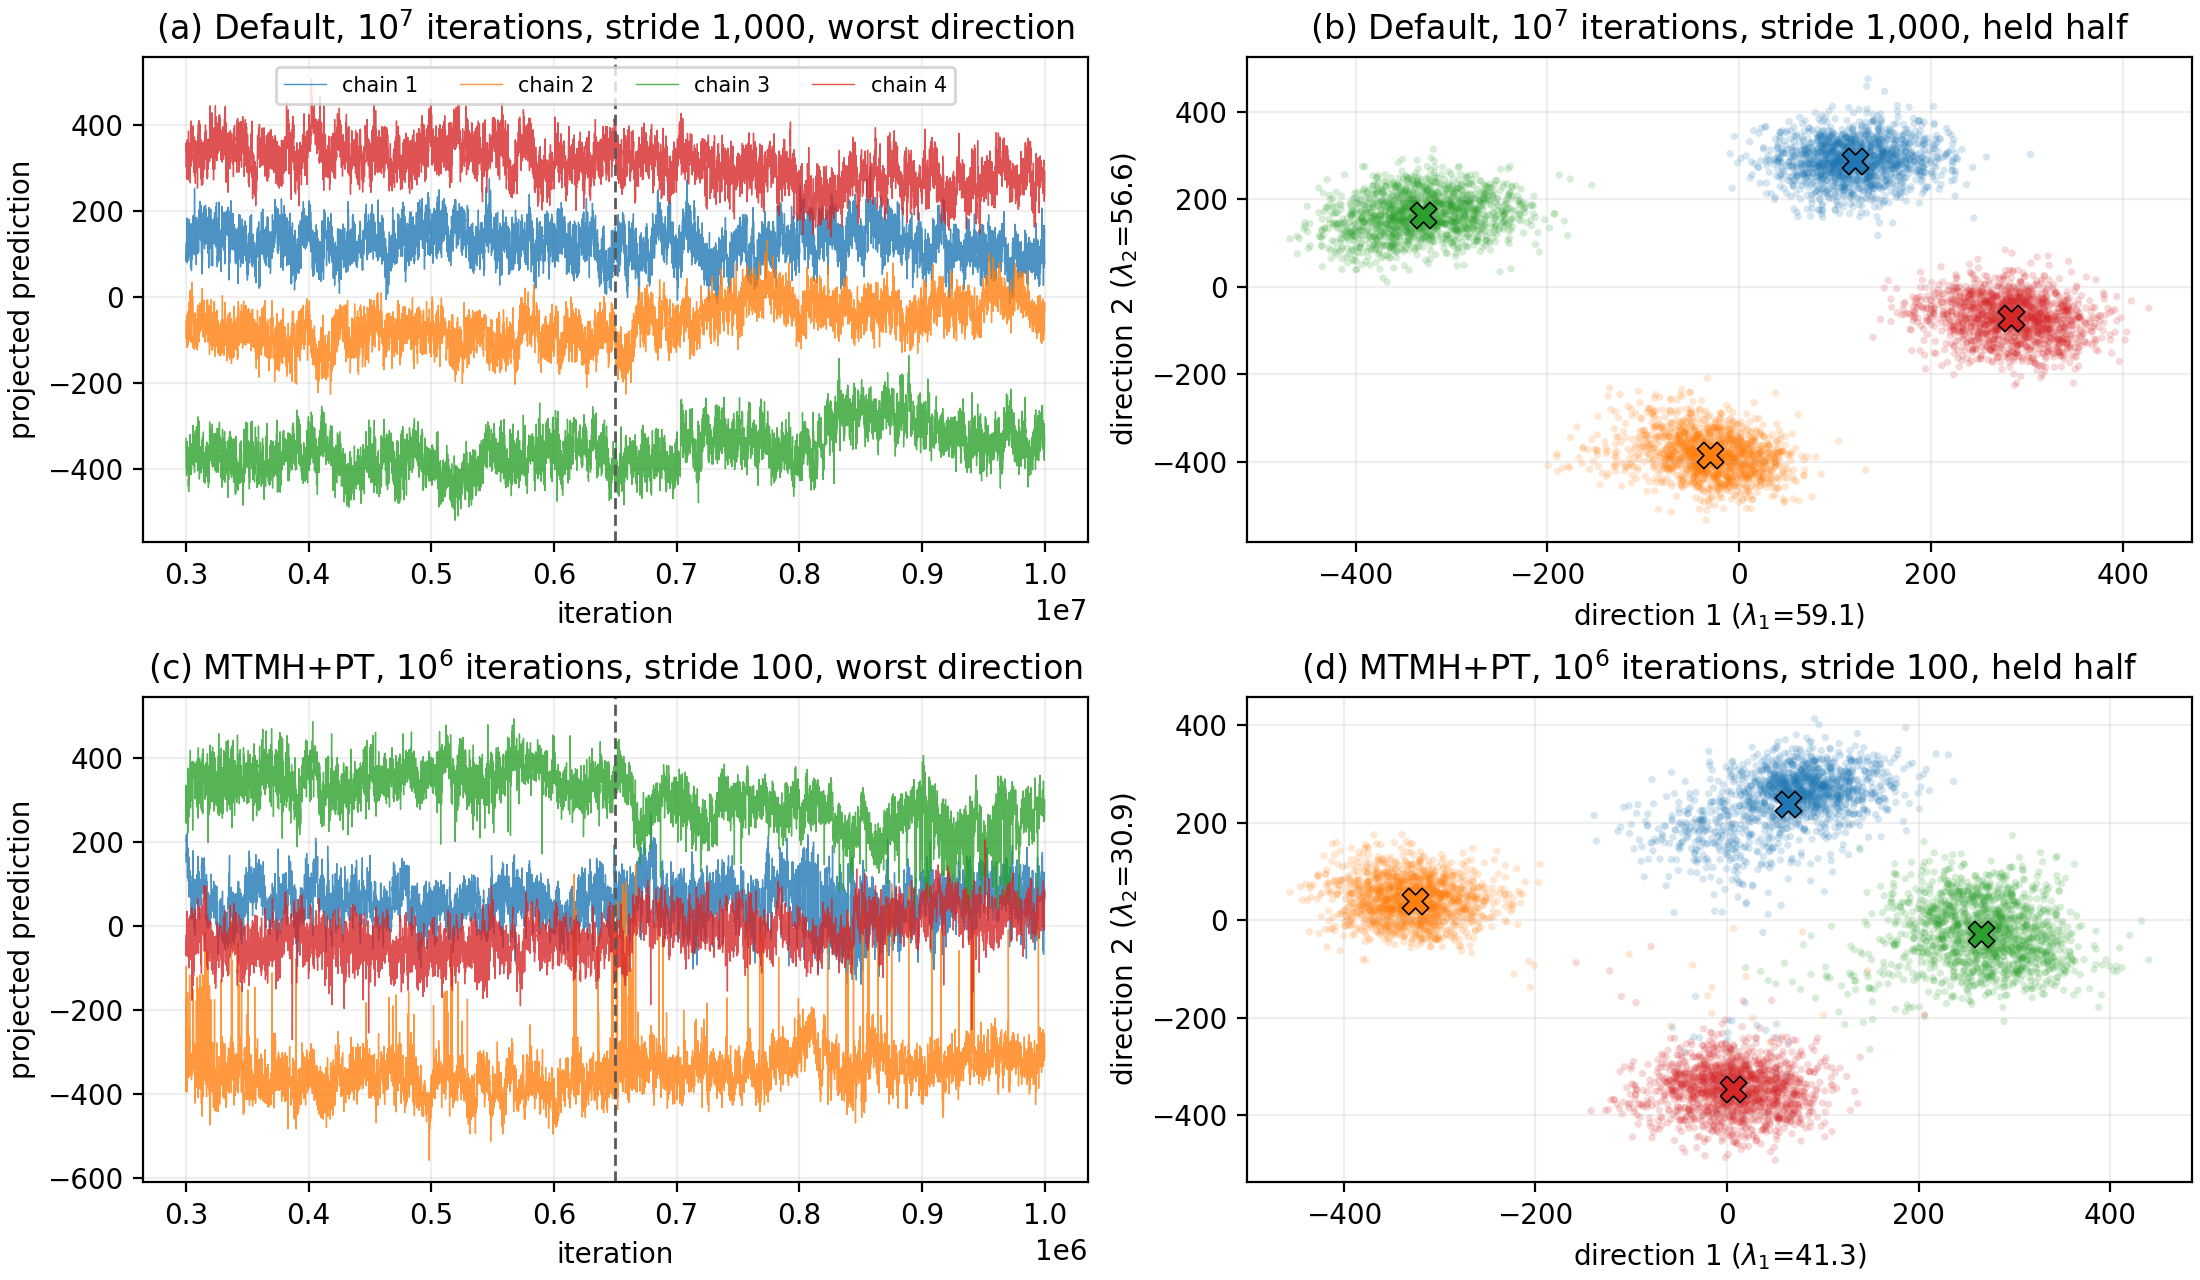
\includegraphics[width=\linewidth]{long_pt_worst2.png}
\caption{SeoulBike run 0, thinned records after the first 30\% is discarded; upper row Default ($10^7$ iterations), lower row MTMH+PT ($10^6$ iterations). (a,c) Predictions of all four chains projected onto the leading generalized eigenvector $v_1$; the dashed line ends the first half, on which the directions are fitted. (b,d) Second-half draws projected onto $v_1$ and $v_2$; crosses mark the chain centroids. Each record has its own axes.}
\label{fig:long-worst}
\end{figure}

\textbf{Trajectories.} Figure~\ref{fig:long-trace} and Table~\ref{tab:long-traj} follow the whole run.
\begin{itemize}
\item The log posterior rises in every chain over the first half. Between the fifth and tenth $10^5$-iteration deciles, chain~1 stays within 10 nats, and chains 2--4 gain 59, 28 and 139 nats.
\item In the last decile, the four chain means span 118 nats.
\item $\sigma$ decreases from about 155 to 132--137, and the total number of splits grows from about 315 to 350--375.
\item The test RMSE of decile-mean predictions ranges from 240 to 306, with no common trend.
\item Mean adjacent exchange acceptance falls from 0.40 in the first chunk to 0.28--0.30 in the last. The ladder was searched for the 0.4 target on a 1,000-row pilot.
\end{itemize}

\begin{figure}[h]
\centering
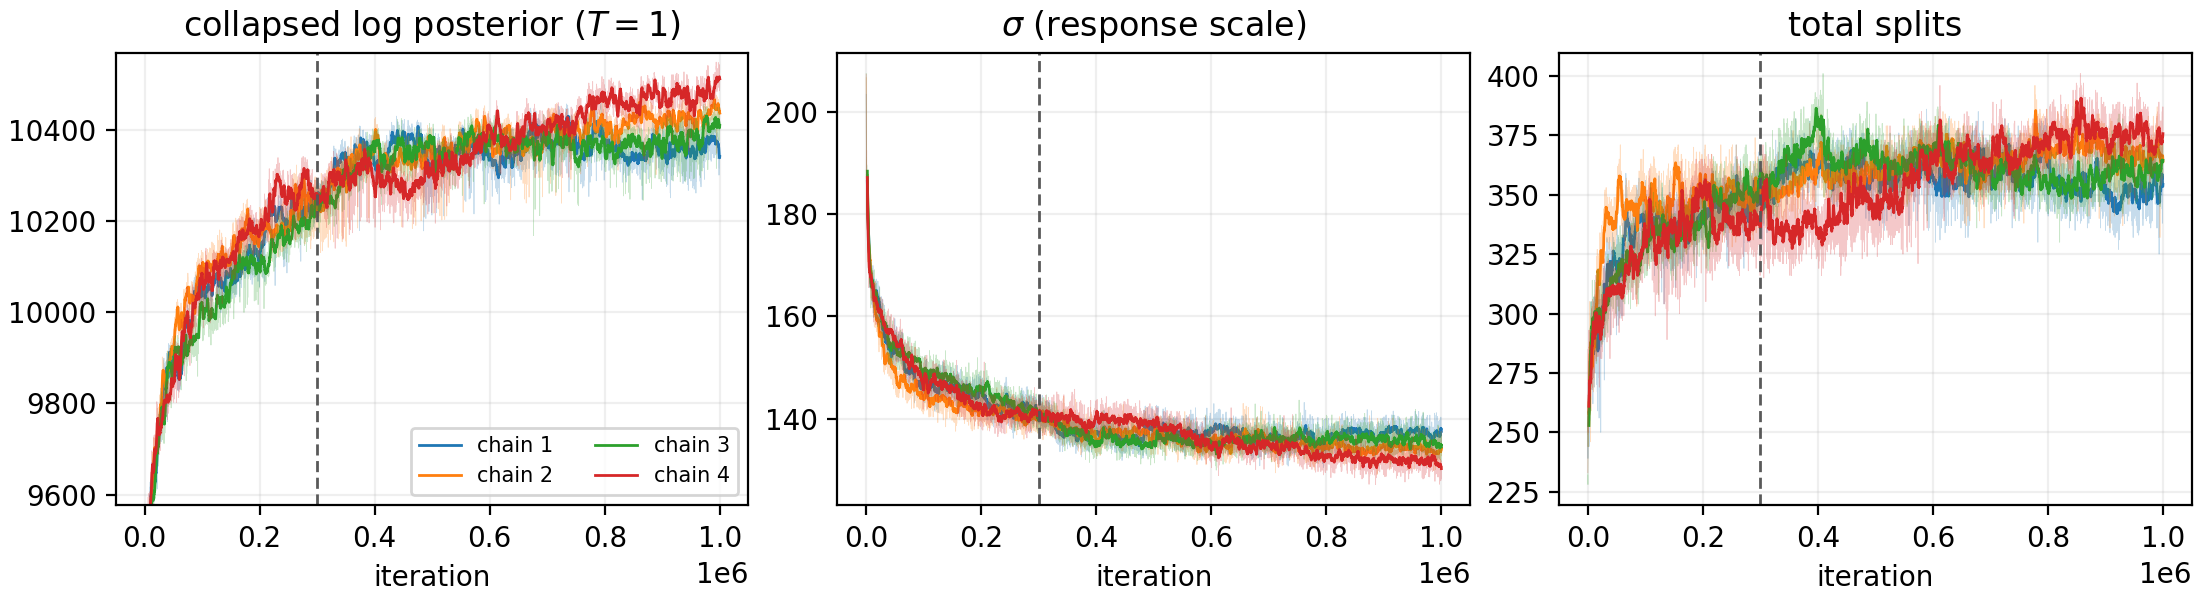
\includegraphics[width=\linewidth]{long_pt_traces.png}
\caption{Long MTMH+PT chains, SeoulBike run 0, every 100th iteration (faint) with a 20-draw moving average. The dashed line marks the end of the discarded first 30\%.}
\label{fig:long-trace}
\end{figure}

\begin{table}[h]
\centering
\small
\caption{Long MTMH+PT chains, SeoulBike run 0: decile means (D1, D5, D10 are iterations 1--100k, 400k--500k and 900k--1M). The log posterior is collapsed and evaluated at $T=1$; $\sigma$ and RMSE are on the response scale.}
\label{tab:long-traj}
\begin{tabular}{lccccccccccc}
\toprule
 & \multicolumn{3}{c}{log posterior} & \multicolumn{3}{c}{$\sigma$} & \multicolumn{3}{c}{total splits} & \multicolumn{2}{c}{test RMSE} \\
\cmidrule(lr){2-4}\cmidrule(lr){5-7}\cmidrule(lr){8-10}\cmidrule(lr){11-12}
Chain & D1 & D5 & D10 & D1 & D5 & D10 & D1 & D5 & D10 & D1 & D10 \\
\midrule
1 & 9{,}834 & 10{,}358 & 10{,}360 & 155.6 & 136.7 & 137.3 & 317 & 361 & 350 & 273 & 248 \\
2 & 9{,}868 & 10{,}339 & 10{,}428 & 152.5 & 137.2 & 134.2 & 332 & 359 & 366 & 266 & 276 \\
3 & 9{,}807 & 10{,}353 & 10{,}389 & 156.8 & 135.6 & 135.6 & 311 & 367 & 360 & 250 & 291 \\
4 & 9{,}831 & 10{,}285 & 10{,}478 & 156.6 & 139.7 & 131.8 & 309 & 344 & 375 & 254 & 297 \\
\bottomrule
\end{tabular}
\end{table}

\textbf{Summary.} After $10^6$ iterations the four chains are not stationary: the log posterior is still rising in three of them, and $\sigma$ is still falling in two. Their pointwise agreement is better than that of the $10^7$-iteration Default chains, but not better than that of the production PT chains, and remains far from 1. They cannot serve as a reference posterior for SeoulBike. This agrees with the position of SeoulBike in Table~\ref{tab:paper}, where it has the third-largest $\kappa$ among the paper settings.

\section{Conclusions}
\begin{enumerate}
\item Collapsing the leaves makes the log-likelihood cost of a structural change proportional to $\kappa=n/(1-R^2)$ per unit of unexplained variance. The tree prior, the proposal ratio and the leaf term do not grow with $\kappa$.
\item Across 48 settings, $\kappa$ orders Default mixing difficulty ($\rho=0.89$). The regression coefficients of $n$ and of the noise fraction agree within their standard errors when $1-R^2_{\mathrm{CV}}$ is used. Responses with equal $\kappa$ give equal $\Rhat$ whether observed or semi-synthetic.
\item $\kappa$ can be computed from a cross-validated fit before running MCMC. The same ordering appears in the $10^7$-iteration chains, and $\kappa$ predicts the settings that remain unresolved.
\end{enumerate}

\textbf{Limitations.}
\begin{itemize}
\item The derivation is a scale argument. It assumes comparable barrier depths $\delta^\ast$ across datasets and does not give mixing times.
\item $\Rhat$ is measured at $10^4$ iterations for 48 settings and at $10^7$ for twelve.
\item The controlled settings use three runs, and acceptance rates use one chain per setting.
\item The relation is a monotone ordering with scatter, not a calibrated prediction. Near $\kappa\approx1.6\times10^4$, for example, $\Rhat$ ranges from 1.06 (CCPP sweep, $n=1{,}000$) to 1.30 (Airfoil).
\item The cross-validated noise fraction depends on the gradient-boosting fit. It overstates the noise fraction when many predictors are irrelevant, as in the DART settings.
\end{itemize}

\textbf{Files.} Scripts and summaries are in \texttt{diagnosis/kappa\_note/} (branch \texttt{kappa-note}). Long-chain output is in \texttt{/scratch/e1377027/long\_pt/fixed100\_SeoulBike/} on Vanda; the runner is \texttt{hpc\_opt/long\_pt.py}.

\begin{thebibliography}{9}
\bibitem[Tan et al.(2024)]{tan2024computational}
Y.~S. Tan, O.~Ronen, T.~Saarinen and B.~Yu.
\newblock On the computational efficiency of Bayesian additive regression trees: an asymptotic analysis.
\newblock arXiv:2406.19958, 2024.
\end{thebibliography}

\end{document}
